% !TEX root = ../../../main.tex
% !TEX encoding = UTF-8 Unicode
% !TEX encoding = UTF-8

\section{Ausgewählte Projekt-Beispiele - KL}
% \textit{Autor: Klaus Landsdorf}

\label{section_projekt_beispiele}
Die DFG wählt, in einem jährlichen Bewerbungsdurchgang, die besten vier Projekte für eine Förderungsperiode aus.\footnote{Für Auskünfte steht Ihnen aktuell Frau Holzer (E-Mail: Angela.Holzer@dfg.de Tel.: 0228/885-2344) Rede und Antwort \url{http://www.dfg.de/formulare/12_13/12_13_de.pdf}} Diese vier Projekte wurden bisher mit EUR 50.000 für die detaillierte Planungsphase und deren Umsetzung ausgestattet. In einem zweiten Förderzeitraum, von maximal fünf Jahren, wurden zwei der vier Projekte mit jeweils EUR 250.000 pro Jahr ausgestattet.
Insgesamt entspricht das einem Fördervolumen von gut EUR 1,3 Mio. für ein integriertes Informationsmanagement.
Die folgenden Projekte wurden im Zeitraum 2005 - 2010 durchgeführt und haben ihre Erfahrungen in Publikationen bereitgestellt.\footnote{\cite{kerres_hochschulen_2005}}

Als Bestätigung dieser Zahlen weist die TU München mehr als fünfzig Mitarbeiterinnen und Mitarbeiter im Projekt aus. Zu ihrem integrierten Informationsmanagement bekam das Projekt insgesamt ca. EUR 2,5 Mio. Förderung. Die TU München stellte dazu selbst weitere Sondermittel aus dem Erneuerungsprojekt InnovaTUM zur Verfügung.\footnote{\cite{bode_informationsmanagement_2010}}

In diesem Abschnitt werden zwei Referenzprojekte des integrierten Informationsmanagements mit DFG Förderung betrachtet, da hierfür einige Zahlen bekannt sind, mit denen eine Überlegung für die Hochschule Emden/Leer angestellt werden kann.

% \clearpage

Das erste Referenzprojekt des integrierte Informationsmanagements, ist das Münster Information System for Research and Organization (MIRO) der Westfälischen Wilhelms-Universität (WWU) Münster. Die ersten Bemühungen starteten im Jahr 2003 und wurden in den folgenden Jahren vorangetrieben. Im Jahre 2005, sowie zum abschließenden Berichtsstand der WWU 2013, existierten 15 Fachbereiche an der WWU. Die 130 Studienfächer sanken in diesem Zeitraum auf 110. Auch die ca. 39.000 Studierenden sind im Jahr 2013 auf ca. 37.000 Studierende gesunken.

% \clearpage

An der WWU waren zum Zeitpunkt der Antragstellung etwa 5.000 Personen beschäftigt, davon 600 Professoren, 2.600 wissenschaftliche und 1.800 weitere Mitarbeiter. Im Jahr 2013 sind über 550 Professoren und ca. 3800 wissenschaftliche Beschäftigte an der WWU.\footnote{\cite{vogl_bericht_2013}}

\newpage

\begin{itemize}
	\item Erreichtes
	\begin{itemize}
		\item Flexible IT-Architektur - SOA / SOI
		\item Identitätsmanagement (MORITZ)
		\item Digitlaes Publizieren
		\item Enterprise Content Management (ECM) (Alfresco, SAN, Oracle Cluster)
		\item Mobile Dienste (Alfresco)
		\item Portalinfrastruktur (Apache Webserver, JBoss, Oracle Cluster)
	\end{itemize}
\end{itemize}

% \newpage
		
\begin{itemize}	
	\item Aufwand
	\begin{itemize}
		\item 16 wissenschaftliche Mitarbeiter - 8 davon DFG gefördert
		\item über einen Zeitraum von sechs Jahren
		\item Finanzmittel
		\begin{itemize}
			\item beträchtliche Finanzmittel durch das Rektorat der Universität
			\item vor allem notwendige Sachausgaben
		\end{itemize}
	\end{itemize}
\end{itemize}

\textit{„Nach über zehn Jahren ist festzuhalten, dass sich die Strukturen in der Informationsverarbeitung und -versorgung sehr bewährt haben. Den Verantwortlichen ist es gelungen, die Informationsverarbeitung und -versorgung in Münster auf einen beachtlichen Stand der Technik und Organisation zu bringen.“}\footnote{\cite{bode_informationsmanagement_2010}}

% \clearpage

In der Tabelle \ref{tab_minimale_investition_munster} können die Zahlen der DFG-Förderung für die WWU aufgeschlüsselt werden.
Die Annahme der Personalkosten von 75 \%, leitet sich aus einem Bericht\footnote{\autocite{schuelein_2009}} der Kosten in fertigenden Unternehmen und der Automobilbranche ab, da es im Zeitrahmen der Arbeit nicht möglich war belegbare Zahlen für Hochschulen zu ermitteln. 

\begin{table}[h!]
	\begin{tabularx}{\textwidth}{l|l}
		\hline
		\textbf{Kostenaufteilung Annahme MIRO} & \textbf{Betrag in EUR}\\
		Gesamtvolumen über 5 Jahre & 1.300.000\\
		Personalkosten IT ca. 75 \% & 975.000\\
		Kosten pro Projektmitarbeiter (16) & 56.875 (ca. 5.080 / Monat)\\ 
		Sonstige Kosten (unbekannt) & 325.000 (ca. 65.000 / Jahr)\\
		\hline
    \end{tabularx}
    \caption{Annahme der minimalen Investition in Münster}
    \label{tab_minimale_investition_munster}
\end{table}

Die geschätzten Kosten der Projektmitarbeiter der Tabelle \ref{tab_minimale_investition_munster} passen zu den Angaben der DFG-Sätze 2015, worin ein/e Doktorandin/Doktorand und Vergleichbare EUR 5.050 monatlich verdienen und Sonstige(r) wissenschaftliche(r) Mitarbeiterinnen oder Mitarbeiter EUR 4.250 Vergütung erhalten.\footnote{Vgl. Tabelle \ref{tab_ubersicht_lohne}} 

\clearpage

Der Mittelwert von der Professur Vergütung bis zum angestellten Mitarbeiter liegt sogar etwas höher bei ca. EUR 5.240 monatlicher Vergütung.

Ein weiteres Projekt des integrierten Informationsmanagements ist das „Karlsruher Integriertes InformationsManagement“ (KIM).
KIM ist im Ansatz eine dienstorientierte Föderation, in der die jeweiligen Fachbereiche sich an bestimmte Schnittstellen 
halten und selbst die Dienste in ihrer bevorzugten Art und Programmierung zur Verfügung stellen. Dabei wurde ein hoch komplexes, aber nach eigenen Angaben sehr flexibles System, im Rahmen der fünf Jahre DFG Förderung, geschaffen.\footnote{\cite{bode_informationsmanagement_2010}}
Die Abbildung \ref{fig_ubersicht_karlsruhe} zeigt am besten, was in diesem Projekt erreicht wurde, da ein schriftliche Beschreibung den Rahmen dieser Arbeit überschreiten würde.

% \newpage

\begin{figure}[h!]
	\centering
	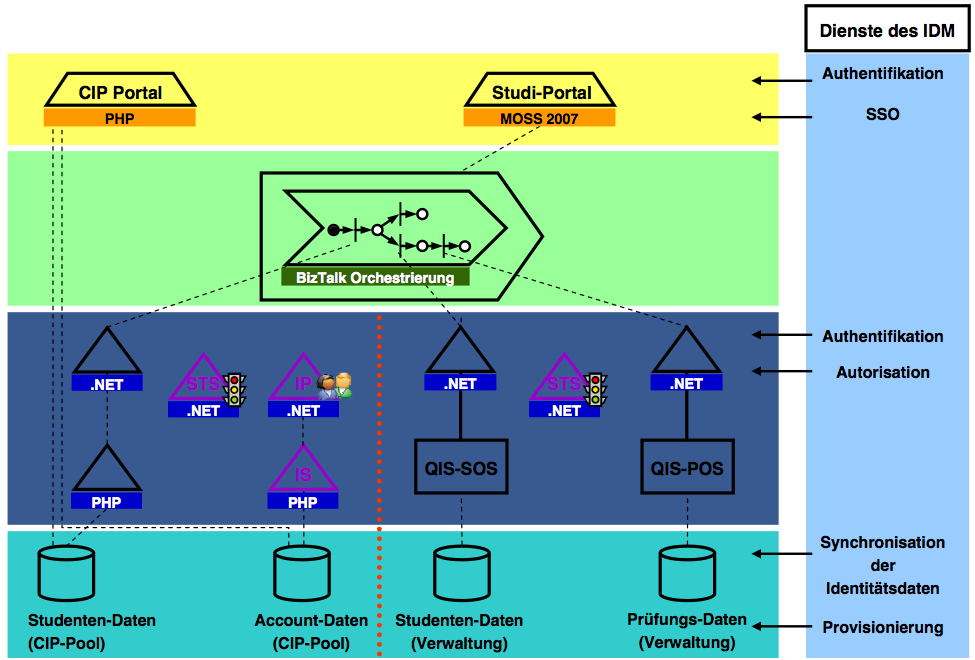
\includegraphics[width=0.75\textwidth]
	{kapitel/gruppe4_2/bilder/ubersicht_karlsruhe}
	\caption{Erreichtes im Überblick für Karlsruhe, nach Juling Best Practice Workshop 2008}
	\label{fig_ubersicht_karlsruhe}
\end{figure}

Besonders gut sind in der Abbildung \ref{fig_ubersicht_karlsruhe} die einzelen unabhängigen Systeme zu erkennen, die von den einzelnen Fachbereichen gepflegt und angeboten werden. 

% \newpage

An der Universität Karlsruhe studieren (Stand 02/2014) ca. 24.500 Studenten, ca. 9500 Mitarbeiter davon 346 Professoren, mit Einnahmen von EUR 795 Mio. wovon Drittmittel EUR 339 Mio. betragen. Die Landesmittel sind mit EUR 212 Mio. und die Bundesmittel mit EUR 349 Mio. angegeben.\footnote{\url{https://www.kit.edu/mediathek/print_forschung/Flyer_KIT_de.pdf}} Den CIO bilden Rektorat und Vorstand.

\begin{figure}[h!]
	\centering
	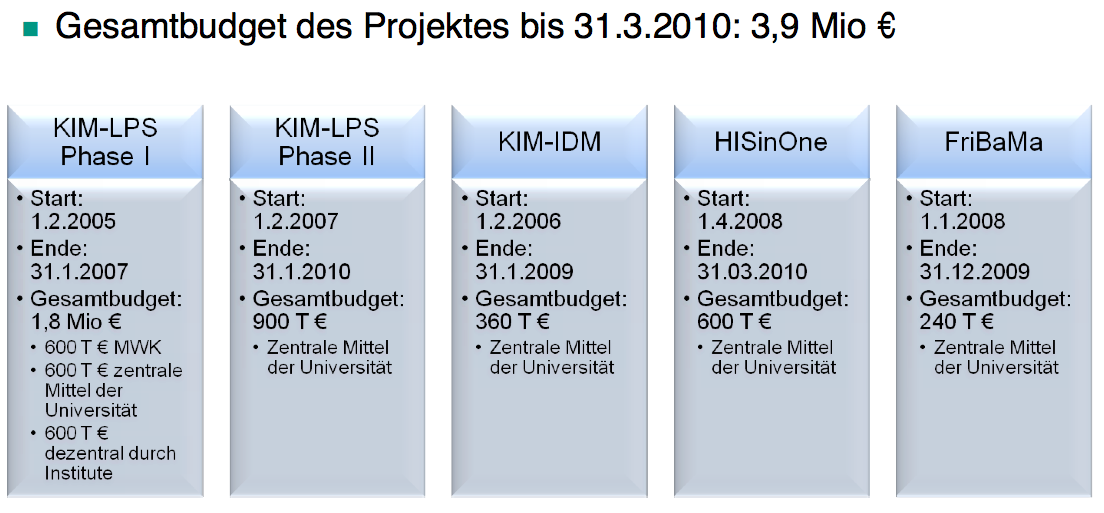
\includegraphics[width=\textwidth]
	{kapitel/gruppe4_2/bilder/uberblick_projekt_KIM}
	\caption{Erreichtes im Überblick für Karlsruhe - Workshop 2008}
	\label{fig_uberblick_projekt_KIM}
\end{figure}

Die Abbildung \ref{tab_minimale_investition_karlsruhe} zeigt die Zahlen des Projektes KIM aus einem Best-Practice Workshop im Jahr 2008.\footnote{\url{http://www.dfg.de/download/pdf/dfg_im_profil/gremien/hauptausschuss/it_infrastruktur/dfg_karlsruhe_juling.pdf}}
Aus diesen bekannt gemachten Werten der Projekte KIM und MIRO, kann nun abgeleitet werden, wieviele Personen an dem Projekt KIM mitgewirkt haben könnten und welche Beträge für sonstige Kosten zur Verfügung standen. Diese Annahme in der Tabelle \ref{tab_minimale_investition_karlsruhe} ist rein fiktiv und dient lediglich dem Vergleich mit dem Projekt MIRO, dass den selben DFG-Förderungen gegenüber steht.

Da in der Berechnung zu kleine Werte für das Personal entstehen und für KIM nicht klar ist wie viele Personen daran genau gearbeitet haben, wird in allen folgenden Tabellen die Position \enquote{Kosten für ein Projektmitarbeiter} angegeben. Dieser Wert kann dividiert auf mehrere Jahre aufgeteilt werden und ergibt die jeweilig mögliche Stellenanzahl der Projektmitarbeiter. Bsp. zu Tabelle \ref{tab_minimale_investition_karlsruhe}: 50 Mitarbeiter für ein Jahr oder zehn Mitarbeiter für fünf Jahre usw. 

\begin{table}[h!]
	\begin{tabularx}{\textwidth}{l|l}
		\hline
		\textbf{Kostenaufteilung Annahme KIM} & \textbf{Betrag in EUR}\\
		Gesamtvolumen über 5 Jahre & 3.900.000\\
		Personalkosten IT ca. 75 \% & 2.925.000\\
		Kosten für ein Projektmitarbeiter (50 möglich) & 58.500 (ca. 4.875 / Monat)\\ 
		Sonstige Kosten (unbekannt) & 975.000 (ca. 81.250 / Jahr)\\
		\hline
	\end{tabularx}
	\caption{Annahme der minimalen Investition in Karlsruhe}
	\label{tab_minimale_investition_karlsruhe}
\end{table}

% \clearpage

Die Hochschule Emden/Leer ist mit 4.626 Studierenden eine kleine Hochschule, für die nun in Tabelle \ref{tab_kostenaufteilung_emden_MIRO} beispielhaft eine fiktive Annahme durch Teilung, aus den Werten des MIRO Projektes, gezeigt wird. Die Grundlage wäre das Minimum, dass dem MIRO Projekt durch seine DFG Förderung zukam.

\begin{table}[h!]
	\begin{tabularx}{\textwidth}{l|l}
		\hline
		\textbf{Kostenaufteilung Annahme KIM} & \textbf{Betrag in EUR}\\
		Gesamtvolumen über 5 Jahre (fiktiv) & 169.000\\
		Personalkosten IT ca. 75 \% & 126.750\\
		Kosten für ein Mitarbeiterjahr (2 möglich) & 63.375 (ca. 5.281 / Monat)\\ 
		Sonstige Kosten (unbekannt) & 42.250 (ca. 8.450 / Jahr)\\
		\hline
	\end{tabularx}
	\caption{Annahme der minimalen Investition in Emden gegenüber MIRO 13 \%}
	\label{tab_kostenaufteilung_emden_MIRO}
\end{table}

% \newpage

Mit EUR 1,3 Mio. bekannten Projektmitteln, hat die Universität Münster mit ca. 37.000 Studierenden und Jahresmitteln von EUR 621 Mio. zu Emden mit EUR 36 Mio. Jahresmittel und ca. 5.000 Studierenden einen Vergleichsanteil, im Bezug auf die Anzahl der Studenten, von 13 \%, also einen möglichen Multiplikator von 0,13.

Sollte man in Emden den Wert des Projektes etwas besser bewerten, kann man die Grundlage für das Minimum aus dem KIM Projekt durch seine DFG Förderung plus die Zuwendungen, durch Zentral Mittel der Universität Karlsruhe, kalkulieren. Damit würde dem Projekt ein finanzielles Volumen wie in Tabelle \ref{tab_kostenaufteilung_emden_KIM1} zustehen.

\begin{table}[h!]
	\begin{tabularx}{\textwidth}{l|l}
		\hline
		\textbf{Kostenaufteilung Annahme KIM 1} & \textbf{Betrag in EUR}\\
		Gesamtvolumen über 5 Jahre (fiktiv) & 169.000\\
		Personalkosten IT ca. 75\% & 126.750\\
		Kosten für ein Mitarbeiterjahr (2 möglich) & 63.375 (ca. 5.281 / Monat)\\ 
		Sonstige Kosten (unbekannt) & 42.250 (ca. 8.450 / Jahr)\\
		\hline
	\end{tabularx}
	\caption{Annahme der minimalen Investition in Emden gegenüber KIM 20 \%}
	\label{tab_kostenaufteilung_emden_KIM1}
\end{table}

Bei einem anzunehmenden Mittelwert von ca. EUR 4.916 für Personal in Emden, würde etwas mehr Geld für die Position Personal benötigt oder es wird eine Stelle weniger oder eine halbe Stelle angesetzt. Mit EUR 3,9 Mio. hat die Universität Karlsruhe mit ca. 25.000 Studierenden und Jahresmittel von EUR 795 Mio.  zu Emden mit EUR 36 Mio. Jahresmittel und ca. 5.000 Studierenden einen Vergleichsanteil, im Bezug auf die Anzahl der Studenten, von 20 \%.

% \clearpage

Als weitere Annahme kann auf den prozentualen Anteilen, aus Einnahmen der Hochschulen und der Anzahl ihrer Mitarbeiter,
ein Multiplikator gebildet werden. Der Anteil der Hochschule Emden/Leer an den Zahlen, Daten und Fakten liegt jeweils bei 5,8 \%  für die Zahlenvergleiche zu Mitarbeitern und Einnahmen der Universität Karlsruhe. Die Berechnungen mit einem passenden Mutliplikator von 0,058 ergeben die Tabelle \ref{tab_kostenaufteilung_emden_KIM2}.

\begin{table}[h!]
	\begin{tabularx}{\textwidth}{l|l}
		\hline
		\textbf{Kostenaufteilung Annahme KIM 2} & \textbf{Betrag in EUR}\\
		Gesamtvolumen über 5 Jahre (fiktiv) & 226.200\\
		Personalkosten IT ca. 75 \% & 169.650\\
		Kosten für ein Mitarbeiterjahr (3 möglich) & 56.550 (ca. 5.281 / Monat)\\ 
		Sonstige Kosten (unbekannt) & 56.550 (ca. 11.310 / Jahr)\\
		\hline
	\end{tabularx}
	\caption{Annahme der minimalen Investition in Emden gegenüber KIM 5,8 \%}
	\label{tab_kostenaufteilung_emden_KIM2}
\end{table}

\clearpage

Auffällig im Vergleich mit anderen Hochschulen und Universitäten, hat die Hochschule Emden/Leer einen geringen Anteil an Drittmitteln zur Verfügung. Der aktuell ausgewiesene Wert von EUR 1,3 Mio\footnote{\url{https://www.hs-emden-leer.de/no_cache/hochschule/zahlen-daten-fakten.html}} liegt in Münster bei EUR 144,1 Mio.\footnote{\url{http://www.uni-muenster.de/profil/zahlen.html}} und in Karlsruhe bei EUR 358 Mio.\footnote{\url{http://www.kit.edu/kit/daten.php}} Drittmitteln. 

\begin{figure}[h!]
	\centering
	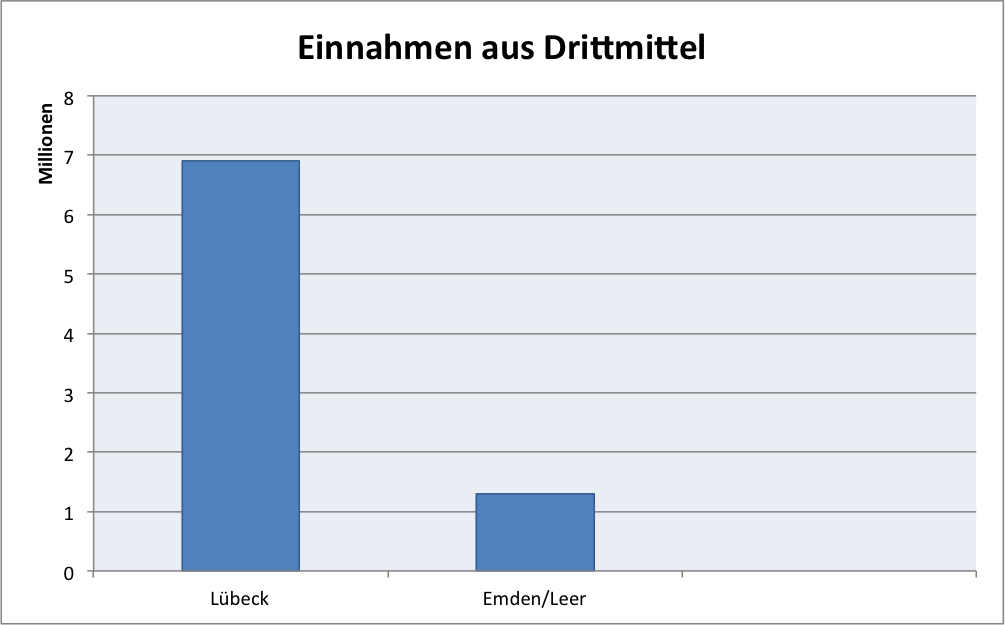
\includegraphics[width=0.75\textwidth]
	{kapitel/gruppe4_2/bilder/EinnhamenDrittmittel}
	\caption{Gegenüberstellung Hochschule Emden/Leer und Lübeck}
	\label{fig_ubersicht_karlsruhe}
\end{figure}

In Prozentzahlen ausgedrückt hat die Hochschule Emden/Leer 3 \% Einnahmen durch Drittmittel, wobei dieser Wert in Münster bei 23 \%, in Karlsruhe bei 42 \% und an der Hochschule Lübeck dem Sechsfachen\footnote{\url{https://www.fh-luebeck.de/hochschule/praesidium/zahlen-daten-fakten/}} entspricht. Hier sollte geprüft werden, ob ein mögliches Potential der Hochschule nicht ausreichend genutzt wird. Als Vergleich liegt die Anzahl der Professoren an der Hochschule Emden/Leer bei 30 \% bzw. ca. 20 \%.

